\documentclass[12pt, a4paper]{article}
% --- Packages ---
\usepackage[utf8]{inputenc}
\usepackage[T1]{fontenc}
\usepackage[french]{babel}
\usepackage{graphicx} % Make sure this is here for images
\usepackage{booktabs}
\usepackage{amsmath}
\usepackage{geometry}
\usepackage{array}
\usepackage{enumitem}
\usepackage{hyperref}
\usepackage{xcolor}
\usepackage{titlesec}
\usepackage{lmodern}
\usepackage{microtype}
\usepackage{fancyhdr}
\usepackage{listings} % Added for code/JSON display
\usepackage[scaled=0.85]{beramono} % Added for a nicer monospaced font

% --- Font Configuration ---
% --- Color Definitions ---
\definecolor{primary}{RGB}{0,51,102}
\definecolor{secondary}{RGB}{102,102,153}
\definecolor{accent}{RGB}{204,0,0}
\definecolor{codegray}{rgb}{0.5,0.5,0.5}
\definecolor{codepurple}{rgb}{0.58,0,0.82}
\definecolor{codeblue}{rgb}{0,0,0.9}
\definecolor{codegreen}{rgb}{0.1,0.6,0.1} % Darker green for comments

% --- Page Geometry ---
\geometry{
  a4paper,
  left=2.5cm,
  right=2.5cm,
  top=2.5cm,
  bottom=2.5cm,
  headheight=15pt
}
% --- Header/Footer Setup ---
\pagestyle{fancy}
\fancyhf{}
\fancyhead[L]{\small Rapport de Stage - Semaine 3 - Jour 1} % Updated
\fancyhead[R]{\small Zakaria el Khaldi}
\fancyfoot[C]{\thepage}
\renewcommand{\headrulewidth}{0.4pt}
\renewcommand{\footrulewidth}{0.4pt}
% --- Title Formatting ---
\titleformat{\section}
  {\normalfont\Large\bfseries\color{primary}}
  {\thesection}{1em}{}
\titleformat{\subsection}
  {\normalfont\large\bfseries\color{secondary}}
  {\thesubsection}{1em}{}
\titleformat{\subsubsection}
  {\normalfont\normalsize\bfseries\color{accent}}
  {\thesubsubsection}{1em}{}
% --- List Formatting ---
\setlist[itemize]{leftmargin=*, nosep}
\setlist[enumerate]{leftmargin=*, nosep}
% --- Hyperlink Setup ---
\hypersetup{
  colorlinks=true,
  linkcolor=primary,
  urlcolor=secondary,
  citecolor=accent
}

% --- Listings Setup for JSON ---
\lstdefinestyle{json}{
    language=json,
    basicstyle=\ttfamily\footnotesize,
    numbers=left,
    numberstyle=\tiny\color{codegray},
    stepnumber=1,
    numbersep=5pt,
    backgroundcolor=\color{white!95!black}, % Very light gray background
    showspaces=false,
    showstringspaces=false,
    showtabs=false,
    frame=tb, % Top and bottom frame
    framextopmargin=3pt,
    framexbottommargin=3pt,
    rulecolor=\color{black!30!white},
    tabsize=2,
    captionpos=b,
    breaklines=true,
    breakatwhitespace=false,
    stringstyle=\color{codepurple},
    commentstyle=\color{codegreen},
    keywordstyle=\color{codeblue}, % For true, false, null
    morestring=[b]",
    literate=
     *{0}{{{\color{codeblue}0}}}{1}
      {1}{{{\color{codeblue}1}}}{1}
      {2}{{{\color{codeblue}2}}}{1}
      {3}{{{\color{codeblue}3}}}{1}
      {4}{{{\color{codeblue}4}}}{1}
      {5}{{{\color{codeblue}5}}}{1}
      {6}{{{\color{codeblue}6}}}{1}
      {7}{{{\color{codeblue}7}}}{1}
      {8}{{{\color{codeblue}8}}}{1}
      {9}{{{\color{codeblue}9}}}{1}
      {:}{{{\color{black}:}}}{1}
      {\{}{{{\color{black}{\{}}}}{1}
      {\}}{{{\color{black}{\}}}}}{1}
      {[}{{{\color{black}{[}}}}{1}
      {]}{{{\color{black}{]}}}}{1}
      {,}{{{\color{black}{,}}}}{1},
}


% --- Title Page Information ---
\title{\Huge\bfseries\color{primary} Rapport de Stage \\ 
      \Large Semaine 3 - Jour 1 : Intégration MongoDB et Déploiement Cloud} % Updated title
\author{\Large Zakaria el Khaldi}
\date{\large Le 20 mai 2025} % Assuming Week 2 ended on Fri, May 17th, Week 3 Day 1 is Mon, May 20th. Adjust if needed.

% --- Document Start ---
\begin{document}
% --- Cover Page ---
\begin{titlepage}
  \centering
  \vspace*{\stretch{0.5}}
  {\Huge\bfseries\color{primary} Rapport de Stage \par}
  \vspace{1cm}
  {\Large\itshape Semaine 3 - Jour 1 : Intégration MongoDB et Déploiement Cloud\par} % Updated title
  \vspace{2cm}
  
  \vspace{2cm}
  {\Large Zakaria el Khaldi\par}
  \vfill
  {\large Le 19 mai 2025\par} % Date of report submission
  \vspace*{\stretch{1}}
\end{titlepage}

% --- Table of Contents ---
\tableofcontents
\thispagestyle{empty}
\newpage

% --- Introduction ---
\section{Introduction}
\thispagestyle{fancy}
Ce rapport quotidien détaille les activités réalisées durant le premier jour de la troisième semaine de stage. Faisant suite à la phase d'analyse et de nettoyage des données de la semaine précédente, cette journée a été consacrée à la structuration et à la pérennisation de ces données. Les objectifs principaux étaient de transférer les données scrappées et nettoyées vers une base de données MongoDB, de déployer cette base dans un environnement cloud pour une meilleure accessibilité, et d'établir la connexion entre l'application en cours de développement et cette base de données distante.

% --- Day's Accomplishments ---
\section{Activités du Jour (Lundi 19 Mai 2025)}

\subsection{Transfert des Données JSON vers MongoDB}
La première tâche de la journée a consisté à migrer l'ensemble des fichiers JSON, contenant les données scrappées et préalablement nettoyées, vers une base de données MongoDB. Chaque fichier JSON a été importé, en créant des collections distinctes pour les différentes catégories de données (par exemple, `course_categories`, `tutorials`). Cette étape a permis de centraliser les données dans un format structuré et interrogeable, facilitant leur future exploitation. Des outils comme `mongoimport` ont été utilisés pour automatiser ce processus.

\subsection{Déploiement de la Base de Données sur MongoDB Atlas}
Afin d'assurer une accessibilité optimale, une scalabilité future et une gestion simplifiée, la base de données MongoDB a été déployée sur MongoDB Atlas, la plateforme de base de données en tant que service (DBaaS) de MongoDB. Ce déploiement dans le cloud (voir Figure \ref{fig:mongodb_atlas_collections}) permet un accès sécurisé et distant aux données, ce qui est crucial pour le développement collaboratif et le futur déploiement de l'application. La configuration initiale du cluster, des utilisateurs et des règles d'accès réseau a été effectuée.

\begin{figure}[htbp]
  \centering
  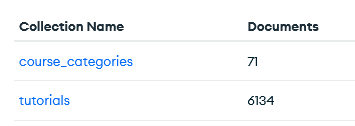
\includegraphics[width=0.9\textwidth]{Screenshot 2025-05-19 234047.png} % !!! REPLACE your_screenshot_filename.png WITH THE ACTUAL FILENAME OF YOUR IMAGE !!!
  \caption{Aperçu des collections}
  \label{fig:mongodb_atlas_collections}
\end{figure}

\subsection{Lecture de la Documentation MongoDB Cloud}
Pour approfondir la compréhension des fonctionnalités de MongoDB Atlas et des meilleures pratiques associées, un temps a été dédié à la lecture de la documentation officielle (\url{https://cloud.mongodb.com}). L'accent a été mis sur les aspects de sécurité, la gestion des clusters, les options de sauvegarde, et les outils de monitoring offerts par la plateforme.

\subsection{Connexion de l'Application à la Base de Données Distante}
La dernière étape de la journée a été d'établir la connexion entre l'application (le backend du projet) et l'instance MongoDB hébergée sur Atlas. Cela a impliqué la mise à jour des configurations de l'application, notamment la chaîne de connexion (connection string) fournie par MongoDB Atlas. Des tests de connectivité ont été réalisés avec succès, confirmant que l'application peut lire et écrire des données dans la base de données distante.

\subsection{Planification pour Demain (Mardi 20 Mai 2025)}
La journée de demain sera axée sur l'exploitation des données désormais accessibles via MongoDB Atlas. Les tâches prévues sont :
\begin{itemize}
  \item Développer les routes d'API et les logiques métier (services) nécessaires pour récupérer les données relatives aux cours et tutoriels depuis MongoDB.
  \item Commencer l'intégration de ces données dans les composants frontend de la section gratuite du site web, en affichant dynamiquement les listes de cours et de tutoriels.
  \item Affiner les requêtes MongoDB pour optimiser la récupération des données.
\end{itemize}

\section{Conclusion}
Cette première journée de la troisième semaine a permis de franchir une étape cruciale dans la gestion des données du projet. Le transfert vers MongoDB et le déploiement sur Atlas offrent une solution robuste et scalable pour le stockage des informations scrappées. La connexion réussie de l'application à cette base distante ouvre la voie au développement des fonctionnalités utilisateur basées sur ce contenu, en commençant par la section gratuite du site web.

\end{document}